\documentclass[twoside]{book}

% Packages required by doxygen
\usepackage{fixltx2e}
\usepackage{calc}
\usepackage{doxygen}
\usepackage[export]{adjustbox} % also loads graphicx
\usepackage{graphicx}
\usepackage[utf8]{inputenc}
\usepackage{makeidx}
\usepackage{multicol}
\usepackage{multirow}
\PassOptionsToPackage{warn}{textcomp}
\usepackage{textcomp}
\usepackage[nointegrals]{wasysym}
\usepackage[table]{xcolor}

% Font selection
\usepackage[T1]{fontenc}
\usepackage[scaled=.90]{helvet}
\usepackage{courier}
\usepackage{amssymb}
\usepackage{sectsty}
\renewcommand{\familydefault}{\sfdefault}
\allsectionsfont{%
  \fontseries{bc}\selectfont%
  \color{darkgray}%
}
\renewcommand{\DoxyLabelFont}{%
  \fontseries{bc}\selectfont%
  \color{darkgray}%
}
\newcommand{\+}{\discretionary{\mbox{\scriptsize$\hookleftarrow$}}{}{}}

% Page & text layout
\usepackage{geometry}
\geometry{%
  a4paper,%
  top=2.5cm,%
  bottom=2.5cm,%
  left=2.5cm,%
  right=2.5cm%
}
\tolerance=750
\hfuzz=15pt
\hbadness=750
\setlength{\emergencystretch}{15pt}
\setlength{\parindent}{0cm}
\setlength{\parskip}{3ex plus 2ex minus 2ex}
\makeatletter
\renewcommand{\paragraph}{%
  \@startsection{paragraph}{4}{0ex}{-1.0ex}{1.0ex}{%
    \normalfont\normalsize\bfseries\SS@parafont%
  }%
}
\renewcommand{\subparagraph}{%
  \@startsection{subparagraph}{5}{0ex}{-1.0ex}{1.0ex}{%
    \normalfont\normalsize\bfseries\SS@subparafont%
  }%
}
\makeatother

% Headers & footers
\usepackage{fancyhdr}
\pagestyle{fancyplain}
\fancyhead[LE]{\fancyplain{}{\bfseries\thepage}}
\fancyhead[CE]{\fancyplain{}{}}
\fancyhead[RE]{\fancyplain{}{\bfseries\leftmark}}
\fancyhead[LO]{\fancyplain{}{\bfseries\rightmark}}
\fancyhead[CO]{\fancyplain{}{}}
\fancyhead[RO]{\fancyplain{}{\bfseries\thepage}}
\fancyfoot[LE]{\fancyplain{}{}}
\fancyfoot[CE]{\fancyplain{}{}}
\fancyfoot[RE]{\fancyplain{}{\bfseries\scriptsize Generated by Doxygen }}
\fancyfoot[LO]{\fancyplain{}{\bfseries\scriptsize Generated by Doxygen }}
\fancyfoot[CO]{\fancyplain{}{}}
\fancyfoot[RO]{\fancyplain{}{}}
\renewcommand{\footrulewidth}{0.4pt}
\renewcommand{\chaptermark}[1]{%
  \markboth{#1}{}%
}
\renewcommand{\sectionmark}[1]{%
  \markright{\thesection\ #1}%
}

% Indices & bibliography
\usepackage{natbib}
\usepackage[titles]{tocloft}
\setcounter{tocdepth}{3}
\setcounter{secnumdepth}{5}
\makeindex

% Hyperlinks (required, but should be loaded last)
\usepackage{ifpdf}
\ifpdf
  \usepackage[pdftex,pagebackref=true]{hyperref}
\else
  \usepackage[ps2pdf,pagebackref=true]{hyperref}
\fi
\hypersetup{%
  colorlinks=true,%
  linkcolor=blue,%
  citecolor=blue,%
  unicode%
}

% Custom commands
\newcommand{\clearemptydoublepage}{%
  \newpage{\pagestyle{empty}\cleardoublepage}%
}

\usepackage{caption}
\captionsetup{labelsep=space,justification=centering,font={bf},singlelinecheck=off,skip=4pt,position=top}

%===== C O N T E N T S =====

\begin{document}

% Titlepage & ToC
\hypersetup{pageanchor=false,
             bookmarksnumbered=true,
             pdfencoding=unicode
            }
\pagenumbering{alph}
\begin{titlepage}
\vspace*{7cm}
\begin{center}%
{\Large 3D Game Programming Assignment 2 }\\
\vspace*{1cm}
{\large Generated by Doxygen 1.8.12}\\
\end{center}
\end{titlepage}
\clearemptydoublepage
\pagenumbering{roman}
\tableofcontents
\clearemptydoublepage
\pagenumbering{arabic}
\hypersetup{pageanchor=true}

%--- Begin generated contents ---
\chapter{Hierarchical Index}
\section{Class Hierarchy}
This inheritance list is sorted roughly, but not completely, alphabetically\+:\begin{DoxyCompactList}
\item Base\+Application\begin{DoxyCompactList}
\item \contentsline{section}{Basic\+Tutorial2}{\pageref{class_basic_tutorial2}}{}
\end{DoxyCompactList}
\end{DoxyCompactList}

\chapter{Class Index}
\section{Class List}
Here are the classes, structs, unions and interfaces with brief descriptions\+:\begin{DoxyCompactList}
\item\contentsline{section}{\hyperlink{class_basic_tutorial2}{Basic\+Tutorial2} }{\pageref{class_basic_tutorial2}}{}
\end{DoxyCompactList}

\chapter{Class Documentation}
\hypertarget{class_basic_tutorial__00}{}\section{Basic\+Tutorial\+\_\+00 Class Reference}
\label{class_basic_tutorial__00}\index{Basic\+Tutorial\+\_\+00@{Basic\+Tutorial\+\_\+00}}
Inheritance diagram for Basic\+Tutorial\+\_\+00\+:\begin{figure}[H]
\begin{center}
\leavevmode
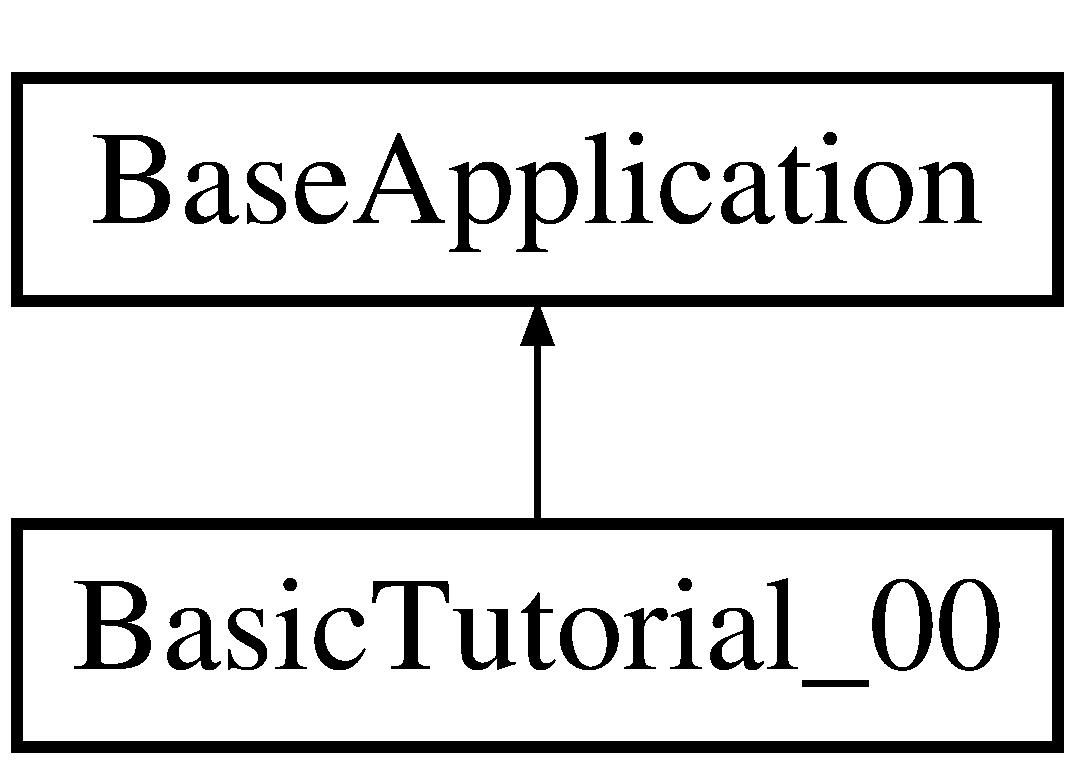
\includegraphics[height=2.000000cm]{class_basic_tutorial__00}
\end{center}
\end{figure}
\subsection*{Public Member Functions}
\begin{DoxyCompactItemize}
\item 
virtual void \hyperlink{class_basic_tutorial__00_a15a3d4673724ec99077ce992f996a550}{create\+Scene} (void)
\begin{DoxyCompactList}\small\item\em Create the specific scene. \end{DoxyCompactList}\item 
virtual void \hyperlink{class_basic_tutorial__00_a84ba95a0d9c9388aa975cf97f19673f0}{create\+Circle\+Of\+Objects} (Ogre\+::\+String object\+Mesh, Ogre\+::\+Real num\+Objects, float circle\+Radius, Ogre\+::\+Scene\+Manager $\ast$m\+Scene\+Mgr, Ogre\+::\+String prefix)
\begin{DoxyCompactList}\small\item\em Create a series of objects that form a circle. \end{DoxyCompactList}\end{DoxyCompactItemize}


\subsection{Member Function Documentation}
\hypertarget{class_basic_tutorial__00_a84ba95a0d9c9388aa975cf97f19673f0}{}\label{class_basic_tutorial__00_a84ba95a0d9c9388aa975cf97f19673f0} 
\index{Basic\+Tutorial\+\_\+00@{Basic\+Tutorial\+\_\+00}!create\+Circle\+Of\+Objects@{create\+Circle\+Of\+Objects}}
\index{create\+Circle\+Of\+Objects@{create\+Circle\+Of\+Objects}!Basic\+Tutorial\+\_\+00@{Basic\+Tutorial\+\_\+00}}
\subsubsection{\texorpdfstring{create\+Circle\+Of\+Objects()}{createCircleOfObjects()}}
{\footnotesize\ttfamily void Basic\+Tutorial\+\_\+00\+::create\+Circle\+Of\+Objects (\begin{DoxyParamCaption}\item[{Ogre\+::\+String}]{object\+Mesh,  }\item[{Ogre\+::\+Real}]{num\+Objects,  }\item[{float}]{circle\+Radius,  }\item[{Ogre\+::\+Scene\+Manager $\ast$}]{m\+Scene\+Mgr,  }\item[{Ogre\+::\+String}]{prefix }\end{DoxyParamCaption})\hspace{0.3cm}{\ttfamily [virtual]}}



Create a series of objects that form a circle. 

A circle is formed by repeatedly rendering the same basic units of objects that are distributed evenly. The objects have varying heights that follow a sine function to produce a wavy effect.


\begin{DoxyParams}{Parameters}
{\em object\+Mesh} & The type of object that forms the circle \\
\hline
{\em num\+Objects} & The number of basic units of objects \\
\hline
{\em circle\+Radius} & The radius of the circle formed by objects \\
\hline
{\em m\+Scene\+Mgr} & The target scene manager\\
\hline
\end{DoxyParams}
\begin{DoxyReturn}{Returns}
void 
\end{DoxyReturn}
\hypertarget{class_basic_tutorial__00_a15a3d4673724ec99077ce992f996a550}{}\label{class_basic_tutorial__00_a15a3d4673724ec99077ce992f996a550} 
\index{Basic\+Tutorial\+\_\+00@{Basic\+Tutorial\+\_\+00}!create\+Scene@{create\+Scene}}
\index{create\+Scene@{create\+Scene}!Basic\+Tutorial\+\_\+00@{Basic\+Tutorial\+\_\+00}}
\subsubsection{\texorpdfstring{create\+Scene()}{createScene()}}
{\footnotesize\ttfamily void Basic\+Tutorial\+\_\+00\+::create\+Scene (\begin{DoxyParamCaption}\item[{void}]{ }\end{DoxyParamCaption})\hspace{0.3cm}{\ttfamily [virtual]}}



Create the specific scene. 

Create the scene of penguins and cube

\begin{DoxyReturn}{Returns}
void 
\end{DoxyReturn}


The documentation for this class was generated from the following files\+:\begin{DoxyCompactItemize}
\item 
source/Tutorial\+Application.\+h\item 
source/Tutorial\+Application.\+cpp\end{DoxyCompactItemize}

%--- End generated contents ---

% Index
\backmatter
\newpage
\phantomsection
\clearemptydoublepage
\addcontentsline{toc}{chapter}{Index}
\printindex

\end{document}
